\chapter{Results}
Using the algorithm described above one is able to produce a NURBS representation of a structure, that has been optimized with respect to predefined boundary conditions. Examples of initial boundary conditions as well as the resulting optimized structures are presented in \autoref{sec:tests}. Additionally the described topology optimization tool enables a less complicated design workflow from the user's point of view. That workflow is described in \autoref{sec:uex}.
\section{Test Cases}
\label{sec:tests}
\todointernal[inline,author=Benni]{Include material saved for each!}
\subsection{Cantilever}
\begin{figure}[H]
\begin{center}
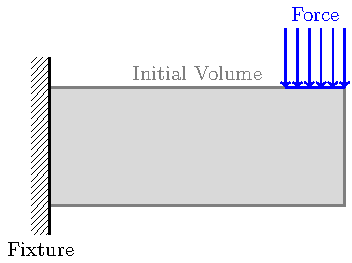
\includegraphics[scale=1]{Pictures/tikzCantilever/canti.pdf}
\end{center}
\caption{Boundary conditions for the test case "Cantilever"}
\end{figure}

\subsection{Bridge}
\begin{figure}[H]
\begin{center}
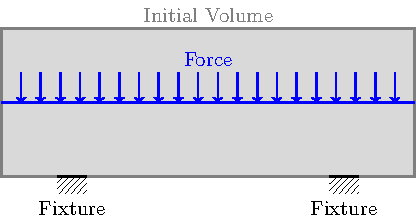
\includegraphics[scale=1]{Pictures/tikzBridge/bridge.pdf}
\end{center}
\caption{Boundary conditions for the test case "Bridge"}
\end{figure}

\subsection{GE Jet Engine Bracket}
\begin{figure}[H]
\begin{center}
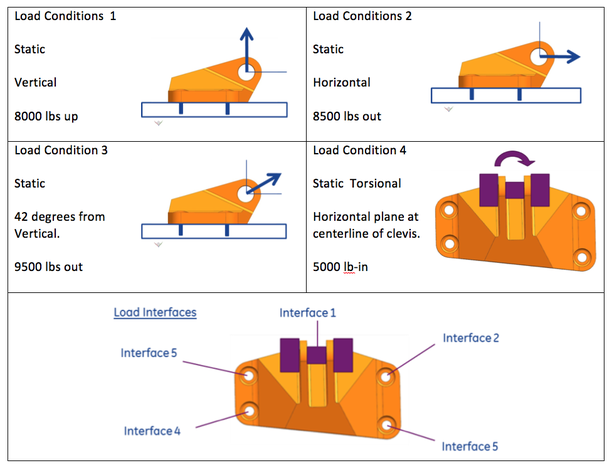
\includegraphics[width=\textwidth]{Pictures/GEbracket.png}
\end{center}
\caption{Boundary conditions and different load cases for test case "GE Bracket". Figure from \cite{GEBracket}}
\end{figure}
Used already optimized design \cite{GEBracketTripon}.


\begin{figure}
\begin{center}
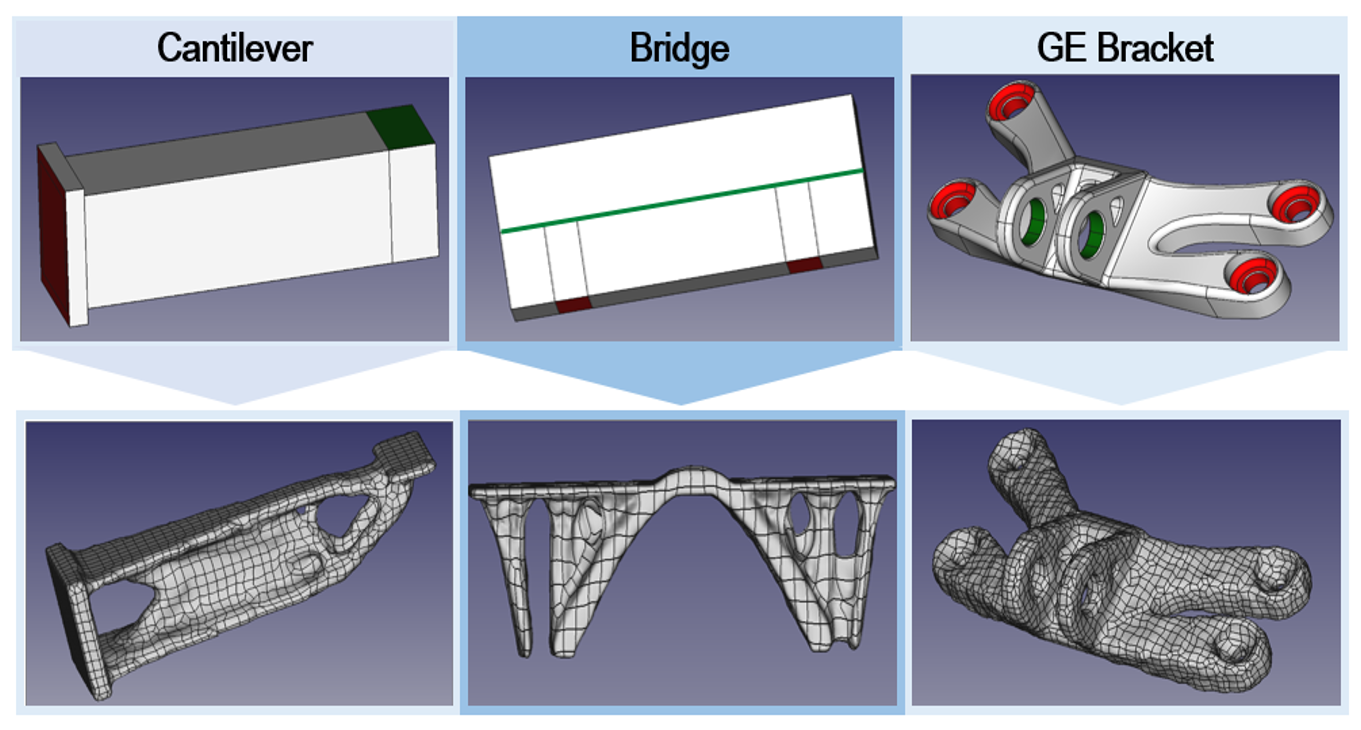
\includegraphics[width = \textwidth]{Pictures/TestCases.png}
\end{center}
\caption{Initial CAD geometry and resulting optimized NURBS geometry for three test cases}
\end{figure}

\section{User Experience}
\label{sec:uex}
\todourgent[inline, author=Benni]{Summarize the the resulting benefits from a user perspective. Put GUI interaction and user documentation here.}